\documentclass[12pt,a4paper, margin=1in]{article}
\usepackage{fullpage}
\usepackage{amsfonts, amsmath, pifont}
\usepackage{amsthm}
\usepackage{amsmath}
\usepackage{geometry}
\usepackage{graphicx}
\usepackage{float}
\graphicspath{{assets/}}

\geometry{
    a4paper,
    % total={210mm,297mm},
    left=10mm,
    right=10mm,
    top=5mm,
    bottom=10mm
}

\author{
    Ahmet Eren Çolak\\
    \texttt{e2587921@ceng.metu.edu.tr}
}

\title{ 
    \textbf{CENG 499 - Introduction to Machine Learning} \\ Homework 2
}

\renewcommand{\thesection}{\arabic{section}}

\begin{document}

\maketitle

\noindent\rule{19cm}{1.2pt}

\tableofcontents

\bigskip
\noindent\rule{19cm}{1.2pt}


\section{Part 2}

\subsection{Dataset 1}

\begin{table}[H]
    \centering
    \begin{tabular}{|c|c|c|c|}
    \hline
    \textbf{ID} & \textbf{C} & \textbf{Kernel}  & \textbf{Accuracy} \\ \hline
    1           & 0.5        & Polynomial       &  0.68 \\ \hline
    2           & 0.5        & RBF              &  1.0  \\ \hline 
    3           & 2          & Polynomial       &  0.69 \\ \hline
    4           & 2          & RBF              &  1.0  \\ \hline
    \end{tabular}
    \caption{Hyperparameter configurations}
\end{table}

I trained and tested all hyperparameters on the same training and test set. Decision boundaries for each hyperparameter
configuration are plotted below.

\subsubsection{Decision Boundaries}

\begin{figure}[H]
    \centering
    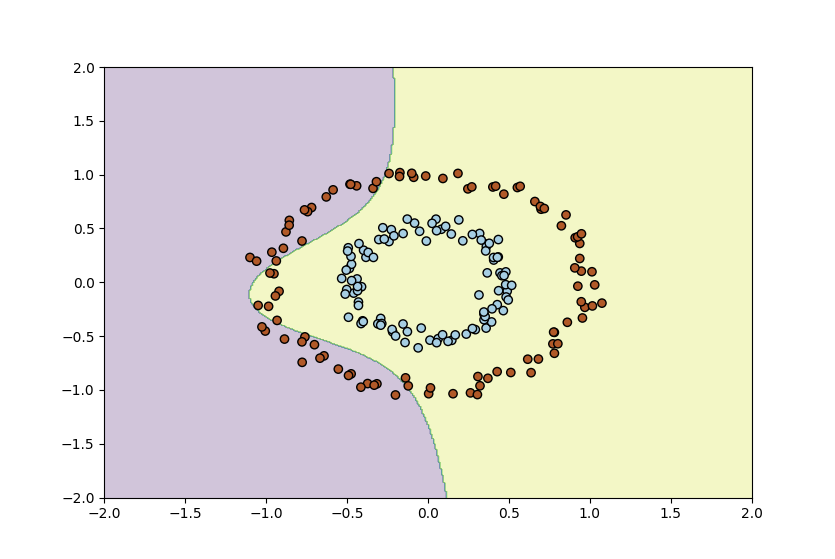
\includegraphics[scale=0.75]{svm-poly-05}
    \caption{Decision boundary of SVM with C = 0.5 and polynomial kernel}
\end{figure}
\begin{figure}[H]
    \centering
    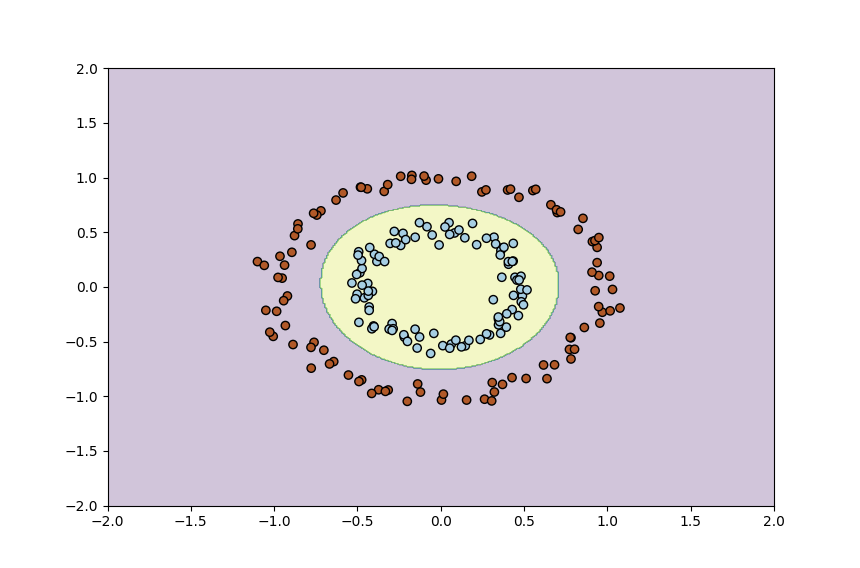
\includegraphics[scale=0.75]{svm-rbf-05}
    \caption{Decision boundary of SVM with C = 0.5 and rbf kernel}
\end{figure}
\begin{figure}[H]
    \centering
    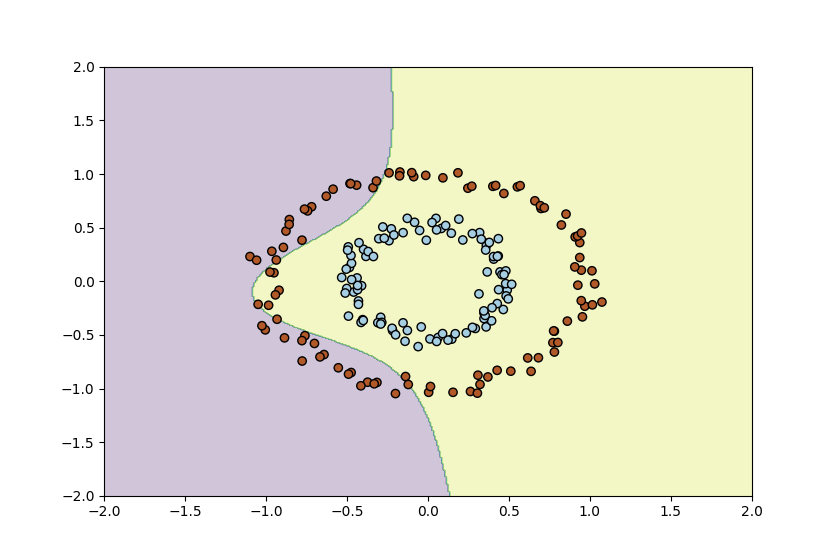
\includegraphics[scale=0.75]{svm-poly-2}
    \caption{Decision boundary of SVM with C = 2 and polynomial kernel}
\end{figure}
\begin{figure}[H]
    \centering
    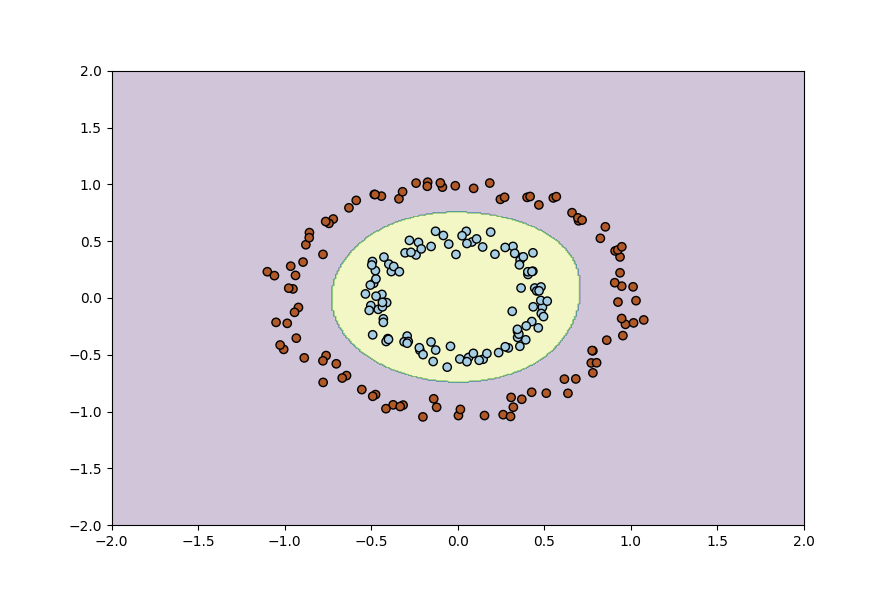
\includegraphics[scale=0.75]{svm-rbf-2}
    \caption{Decision boundary of SVM with C = 2 and rbf kernel}
\end{figure}

\pagebreak

\subsection{Dataset 2}

Hyperparameter configurations on the dataset 1 are kept the same with data set 2.

\begin{table}[H]
    \centering
    \begin{tabular}{|c|c|c|}
    \hline
    \textbf{ID} & \textbf{C} & \textbf{Kernel} \\ \hline
    1           & 0.5        & Polynomial           \\ \hline
    2           & 0.5        & RBF   \\ \hline
    3           & 2          & Polynomial         \\ \hline
    4           & 2          & RBF   \\ \hline
    \end{tabular}
    \caption{Hyperparameter configurations}
\end{table}

I performed cross validation 5 times with 10 splits to find best hyperparameter configurations and plotted accuracy confidence intervals for each configuration. 

\subsubsection{Confidence Intervals}

\begin{figure}[H]
    \centering
    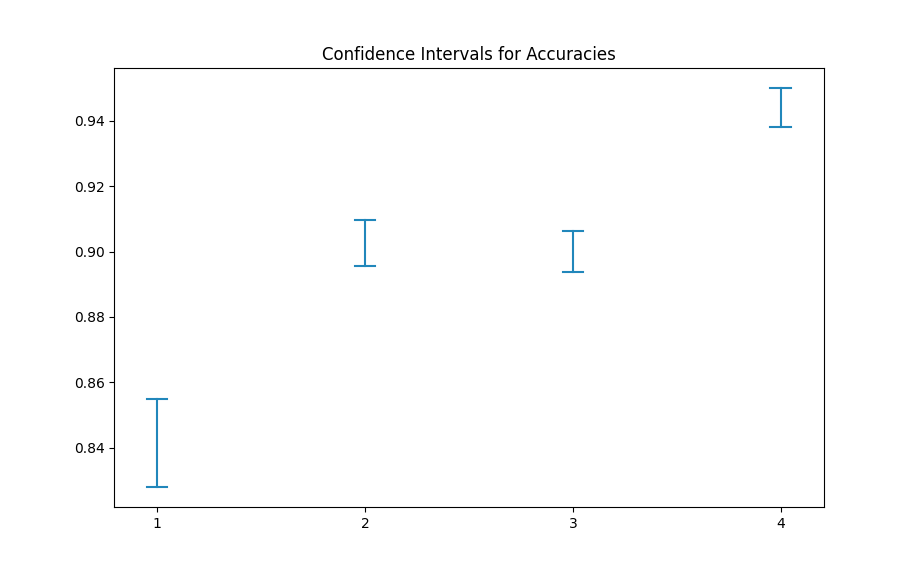
\includegraphics[scale=0.75]{svm_dataset2_ci.png}
    \caption{Accuracy confidence intervals}
\end{figure}

According to the plot, best hyperparameter configuration is the fourth one which is with the C = 2 and rbf kernel.

\pagebreak

\section{Part 3}

I applied nested cross validation to find the best performing algorithm for the credit application dataset, among KNN, SVM, decision trees and random forest algorithms.

\bigskip
\begin{table}[H]
    \centering
    \begin{tabular}{|c|c|l|}
    \hline
    \textbf{ID} & \textbf{Algorithm} & \textbf{Parameter} \\ \hline
    1.1           & KNN        & metric = cosine, \ \ \ \ k = 4           \\ \hline
    1.2           & KNN        & metric = euclidean, k = 4     \\ \hline
    2.1           & SVM        & kernel = linear, C = 1        \\ \hline
    2.2           & SVM        & kernel = rbf, \ \ \ \ C = 1    \\ \hline
    3.1           & Decision Tree        & criterion = entropy           \\ \hline
    3.2           & Decision Tree        & criterion = gini   \\ \hline
    4.1           & Random Forest          & criterion = entropy         \\ \hline
    4.2           & Random Forest          & criterion = gini    \\ \hline
    \end{tabular}
    \caption{Algorithms and hyperparameter configurations}
\end{table}
\bigskip

In the inner cross-validation I picked the best performing hyperparameter for each algorithm. I kept track of how many times a configuration is selected as best for each method.
Since random forest is a stochastic model, I tested random forest algorithm 5 times and computed the mean of 5 accuracy and f1 scores in the inner cross validation.

\subsection{Hyperparameter Search}

\begin{figure}[H]
    \centering
    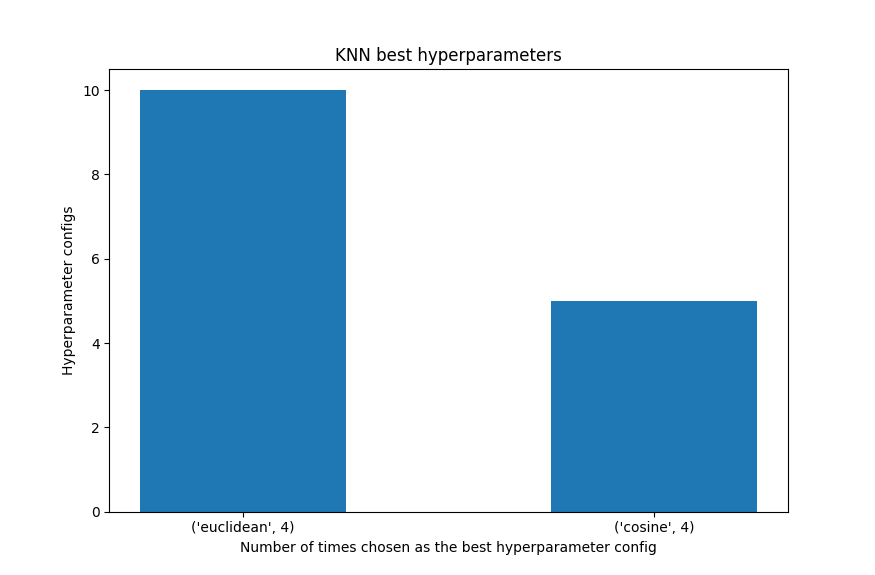
\includegraphics[scale=0.75]{knn-hypr.png}
    \caption{Number of times a hyperparameter is selected as best for KNN}
\end{figure}

\begin{figure}[H]
    \centering
    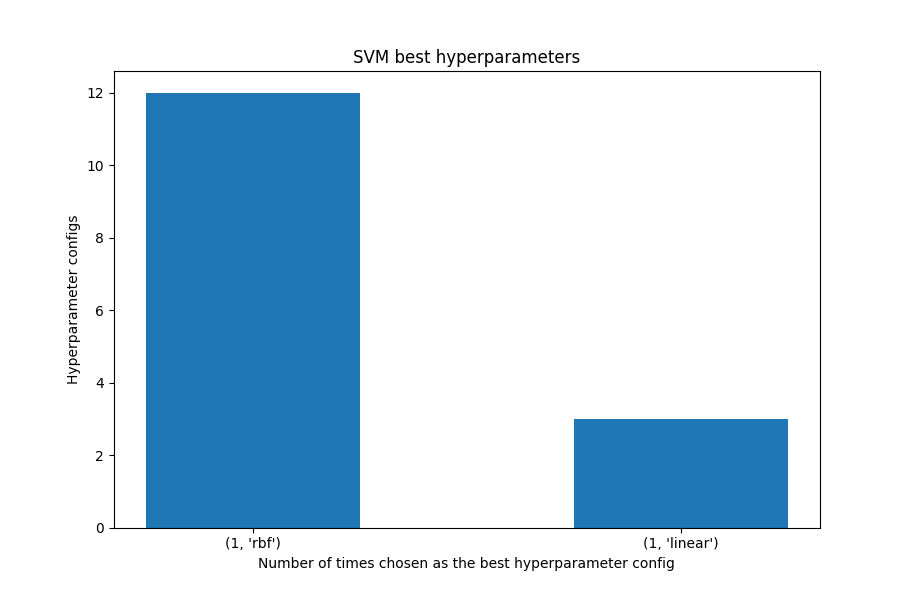
\includegraphics[scale=0.75]{svm-hypr.png}
    \caption{Number of times a hyperparameter is selected as best for SVM}
\end{figure}

\begin{figure}[H]
    \centering
    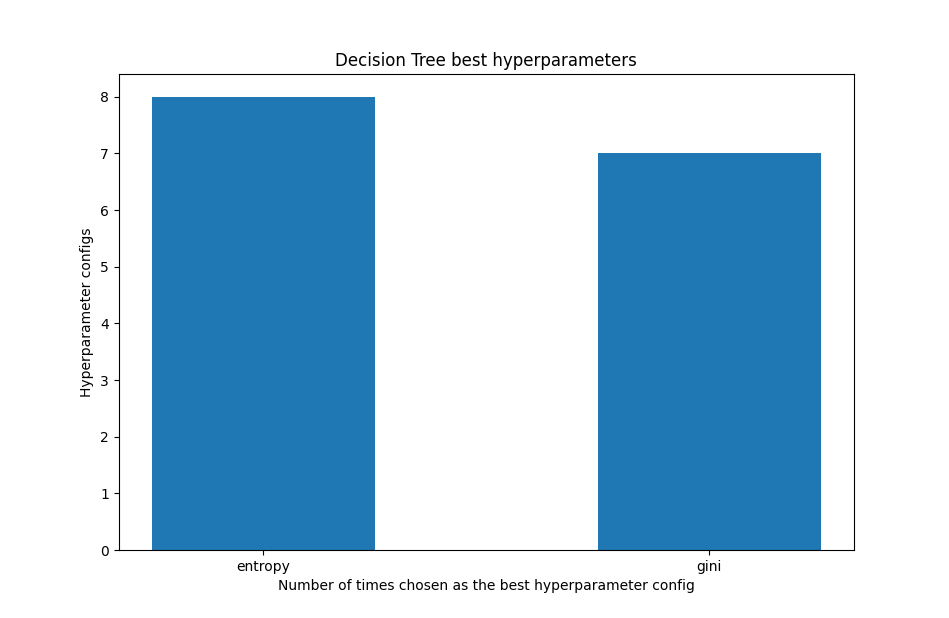
\includegraphics[scale=0.75]{dtree-hypr.png}
    \caption{Number of times a hyperparameter is selected as best for decision tree}
\end{figure}

\begin{figure}[H]
    \centering
    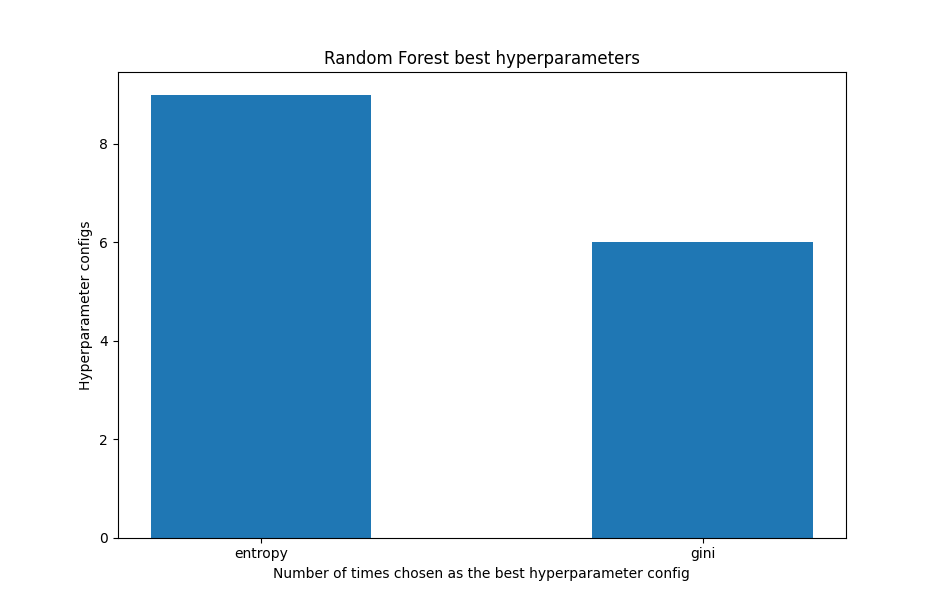
\includegraphics[scale=0.75]{randforest-hypr.png}
    \caption{Number of times a hyperparameter is selected as best for random forest}
\end{figure}

\subsection{Final Evaluation}

In the outer loop of the nested cross validation, I trained and tested best configurations of methods (which I obtained in the inner cross validation) with the outer training and testing folds.
I computed accuracy and f1 scores for each algorithm. As in the inner cross validation, I tested random forest algorithm 5 times and computed mean scores each time.

In the below chart, 1 corresponds to KNN, 2 corresponds to SVM, 3 corresponds to the decision tree and 4 corresponds to the random forest algorithm.

\begin{figure}[H]
    \centering
    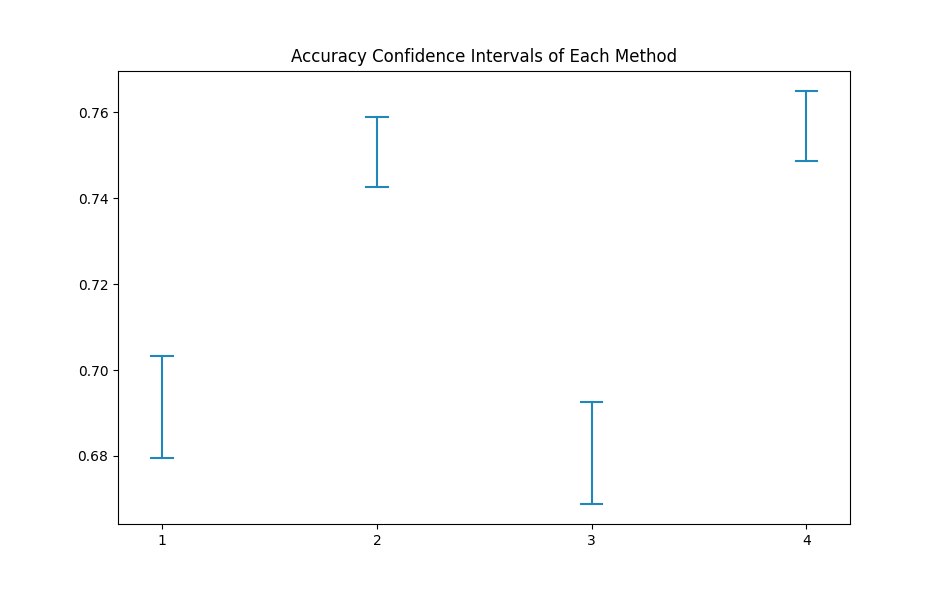
\includegraphics[scale=0.75]{part3-acc-ci-2.png}
    \caption{Accuracy confidence intervals for each algorithm}
\end{figure}

\begin{figure}[H]
    \centering
    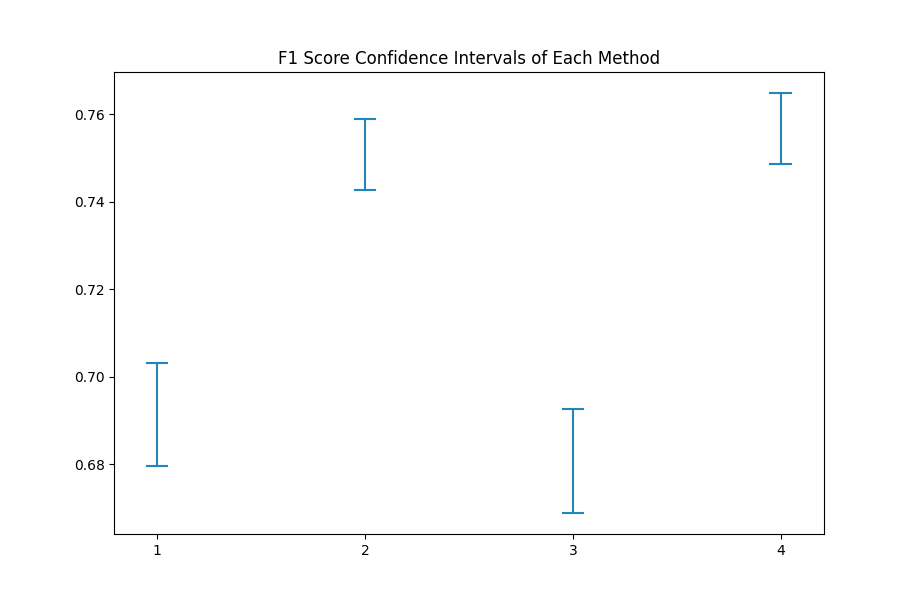
\includegraphics[scale=0.75]{part3-f1s-ci-2.png}
    \caption{F1 score confidence intervals for each algorithm}
\end{figure}
\bigskip

According to the confidence interval charts, best method is the random forest algorithm for this dataset.

\pagebreak

\subsection{Decision Tree Feature Analysis}

Feature importances of the decision tree are as follows:

\begin{small}
\begin{verbatim}
    1   0.14917455 
    2   0.10145336 
    3   0.04544835 
    4   0.06861055 
    5   0.17243175 
    6   0.03775644
    7   0.05490751 
    8   0.02717022 
    9   0.02534325 
    10  0.02110837 
    11  0.04255615 
    12  0.04019985
    13  0.09160992 
    14  0.01699652 
    15  0.02020321 
    16  0.0364606  
    17  0.02917185 
    18  0.0143182
    19  0.00507937 
    20  0.        
\end{verbatim}
\end{small}

Most five important features are the credit amount ($0.17$), status of existing checking account ($0.14$), duration in month ($0.10$), age in years ($0.90$) and purpose ($0.68$) respectively.

\subsection{SVM Support Vector Analysis}
I undid the one hot encoding for both positive and negative support vectors.
\bigskip

Some of the positive class support vectors:
\begin{footnotesize}
\begin{verbatim}
    3.0, 12.0, 4.0, 6.0, 0.0, 0.0, 4.0, 0.0, 0.0, 1.0, 0.0, 0.0, 0.0, 0.0, 0.0, 0.0, 0.0, 0.0, 0.0, 1.0
    0.0, 42.0, 2.0, 2.0, 0.0, 0.0, 4.0, 0.0, 0.0, 0.0, 1.0, 0.0, 0.0, 0.0, 0.0, 1.0, 0.0, 0.0, 0.0, 1.0
    3.0, 36.0, 2.0, 6.0, 0.0, 0.0, 0.0, 0.0, 0.0, 1.0, 0.0, 0.0, 1.0, 0.0, 0.0, 1.0, 0.0, 0.0, 0.0, 0.0
    0.0, 30.0, 0.0, 9.0, 0.0, 0.0, 0.0, 0.0, 0.0, 1.0, 0.0, 0.0, 0.0, 0.0, 2.0, 0.0, 0.0, 0.0, 0.0, 1.0
    1.0, 12.0, 4.0, 1.0, 0.0, 0.0, 2.0, 0.0, 0.0, 1.0, 0.0, 0.0, 0.0, 0.0, 0.0, 0.0, 0.0, 0.0, 0.0, 1.0
    3.0,  6.0, 0.0, 3.0, 0.0, 0.0, 0.0, 1.0, 0.0, 1.0, 0.0, 0.0, 0.0, 0.0, 0.0, 0.0, 0.0, 0.0, 0.0, 1.0
    2.0, 12.0, 1.0, 3.0, 0.0, 0.0, 3.0, 0.0, 0.0, 1.0, 0.0, 0.0, 0.0, 0.0, 0.0, 0.0, 0.0, 0.0, 0.0, 1.0
    1.0, 18.0, 2.0, 9.0, 0.0, 0.0, 2.0, 0.0, 0.0, 1.0, 0.0, 0.0, 0.0, 0.0, 2.0, 0.0, 0.0, 0.0, 0.0, 0.0
    1.0, 18.0, 2.0, 0.0, 0.0, 0.0, 3.0, 0.0, 0.0, 1.0, 0.0, 0.0, 0.0, 0.0, 0.0, 0.0, 0.0, 0.0, 0.0, 0.0
    2.0, 12.0, 2.0, 2.0, 0.0, 0.0, 2.0, 0.0, 0.0, 1.0, 0.0, 0.0, 0.0, 0.0, 2.0, 0.0, 0.0, 1.0, 0.0, 0.0
    2.0, 10.0, 2.0, 4.0, 0.0, 0.0, 3.0, 0.0, 0.0, 1.0, 0.0, 0.0, 0.0, 0.0, 0.0, 0.0, 0.0, 0.0, 0.0, 0.0
    1.0,  9.0, 2.0, 3.0, 0.0, 0.0, 3.0, 0.0, 0.0, 1.0, 0.0, 0.0, 0.0, 0.0, 0.0, 0.0, 0.0, 0.0, 0.0, 1.0
    3.0, 30.0, 2.0, 3.0, 0.0, 0.0, 0.0, 1.0, 0.0, 1.0, 0.0, 0.0, 0.0, 0.0, 2.0, 0.0, 0.0, 1.0, 0.0, 1.0
    3.0, 36.0, 2.0, 3.0, 0.0, 0.0, 0.0, 1.0, 0.0, 1.0, 0.0, 0.0, 0.0, 0.0, 0.0, 0.0, 0.0, 0.0, 0.0, 1.0
    
\end{verbatim}
\end{footnotesize}

Some of the negative class support vectors:
\begin{footnotesize}
    \begin{verbatim}
    1.0, 48.0, 2.0, 3.0, 0.0, 0.0, 3.0, 0.0, 0.0, 1.0, 0.0, 0.0, 0.0, 0.0, 0.0, 0.0, 0.0, 0.0, 0.0, 1.0
    0.0, 24.0, 3.0, 0.0, 0.0, 0.0, 3.0, 0.0, 0.0, 1.0, 0.0, 0.0, 1.0, 0.0, 0.0, 1.0, 0.0, 0.0, 0.0, 1.0
    1.0, 30.0, 4.0, 0.0, 0.0, 0.0, 1.0, 0.0, 0.0, 1.0, 0.0, 0.0, 0.0, 0.0, 0.0, 0.0, 0.0, 1.0, 0.0, 1.0
    1.0, 12.0, 2.0, 0.0, 0.0, 0.0, 2.0, 0.0, 0.0, 1.0, 0.0, 0.0, 0.0, 0.0, 0.0, 0.0, 0.0, 0.0, 0.0, 1.0
    0.0, 48.0, 2.0, 9.0, 0.0, 0.0, 2.0, 0.0, 0.0, 1.0, 0.0, 0.0, 0.0, 0.0, 0.0, 0.0, 0.0, 0.0, 0.0, 1.0
    0.0, 24.0, 4.0, 0.0, 0.0, 0.0, 0.0, 1.0, 0.0, 1.0, 0.0, 0.0, 0.0, 0.0, 0.0, 0.0, 0.0, 0.0, 0.0, 1.0
    0.0, 24.0, 2.0, 3.0, 0.0, 0.0, 3.0, 0.0, 0.0, 1.0, 0.0, 0.0, 0.0, 0.0, 0.0, 0.0, 0.0, 0.0, 0.0, 1.0
    1.0, 24.0, 2.0, 1.0, 0.0, 0.0, 0.0, 1.0, 0.0, 1.0, 0.0, 0.0, 1.0, 0.0, 0.0, 1.0, 0.0, 1.0, 0.0, 0.0
    0.0, 60.0, 3.0, 9.0, 0.0, 0.0, 0.0, 1.0, 0.0, 1.0, 0.0, 0.0, 1.0, 0.0, 0.0, 0.0, 0.0, 0.0, 0.0, 0.0
    1.0, 45.0, 4.0, 3.0, 0.0, 0.0, 2.0, 0.0, 0.0, 1.0, 0.0, 0.0, 0.0, 0.0, 0.0, 0.0, 0.0, 0.0, 0.0, 1.0
    2.0, 18.0, 2.0, 3.0, 0.0, 0.0, 3.0, 0.0, 0.0, 2.0, 0.0, 0.0, 0.0, 0.0, 2.0, 0.0, 0.0, 0.0, 0.0, 1.0
        
    \end{verbatim}
\end{footnotesize}

For 5th, 6th, 9th, 11th, 12th, 13th, 14th, 17th, 19th attributes values are mostly zero among all support vectors.
Also 10th and 20th attribute values consist of mostly 1s. For the 2nd attribute most recurring values are multiples of 6.
\end{document}